\documentclass[conference]{IEEEtran}

\usepackage[T1]{fontenc}
\DeclareUnicodeCharacter{00A0}{ }
\usepackage[utf8]{inputenc}
\usepackage[spanish,es-noshorthands]{babel}
% --- Esta línea obliga a Babel a usar "Tabla" en lugar de "Cuadro" ---
\addto\captionsspanish{\renewcommand{\tablename}{Tabla}}
\usepackage{graphicx}
\usepackage{amsmath}
\usepackage{booktabs}
\usepackage{array}
\usepackage{float}
\usepackage{listings}
\usepackage{xcolor}
\usepackage{caption}
\usepackage{url}

\captionsetup[figure]{font=small}
\captionsetup[table]{font=small}

\definecolor{codeblue}{RGB}{33, 74, 135}
\definecolor{codegreen}{RGB}{34, 139, 34}
\definecolor{codegray}{RGB}{245,245,245}
\definecolor{codecomment}{RGB}{100,100,100}

\lstset{
    language=Python,
    basicstyle=\ttfamily\footnotesize,
    keywordstyle=\color{codeblue}\bfseries,
    commentstyle=\color{codecomment},
    stringstyle=\color{codegreen},
    backgroundcolor=\color{codegray},
    showstringspaces=false,
    breaklines=true,
    frame=single,
    tabsize=4,
    captionpos=b,
    extendedchars=true,
    literate={á}{{\'a}}1 {é}{{\'e}}1 {í}{{\'i}}1 {ó}{{\'o}}1 {ú}{{\'u}}1 {ñ}{{\~n}}1 {Á}{{\'A}}1 {É}{{\'E}}1 {Í}{{\'I}}1 {Ó}{{\'O}}1 {Ú}{{\'U}}1 {Ñ}{{\~N}}1
}

\title{Tarea 03: Implementación de Regresión Logística con PyTorch para Clasificación de Calidad del Vino}

\author{
\IEEEauthorblockN{Jose Miguel Gonzalez Barrantes \qquad Emmanuel Rodríguez Rivas}
\IEEEauthorblockA{
Carné: 2023087564 \qquad Carné: 2023146102 \\
Escuela de Ingeniería en Computación \\
Instituto Tecnológico de Costa Rica \\
Profesor: Steven Andrey Pacheco Portugués \\
Curso: IC6200 Inteligencia Artificial \\
Fecha: Jueves 9 de abril de 2026
}
}

\begin{document}

\maketitle

\begin{abstract}
En este trabajo se implementó un modelo de regresión logística utilizando PyTorch para clasificar la calidad del vino tinto como buena o mala a partir del dataset \textit{Wine Quality Red} de Kaggle. Primero se realizó un análisis exploratorio de datos para estudiar la estructura del conjunto, revisar tipos de variables, valores nulos, duplicados, distribuciones, valores atípicos y correlaciones. Luego, la variable objetivo original fue transformada a una representación binaria, considerando como vinos buenos aquellos con calidad mayor o igual a 6. Después se seleccionaron las seis variables con mayor correlación absoluta respecto a la clase objetivo, se dividieron los datos en entrenamiento, validación y prueba mediante muestreo estratificado, y se aplicó tratamiento de outliers con IQR junto con estandarización. Finalmente, se definió y entrenó un modelo de regresión logística en PyTorch y se ejecutaron diez experimentos variando la tasa de aprendizaje, el tamaño de batch y la cantidad de épocas. Los resultados mostraron que el mejor experimento según F1 sobre validación fue el experimento 2 (F1 de 0.7440). Al evaluar este modelo final con el conjunto de prueba, se obtuvo un F1 de 0.7596 y una exactitud de 0.7549, demostrando una excelente capacidad de generalización sin sobreajuste.
\end{abstract}

\begin{IEEEkeywords}
Regresión logística, PyTorch, clasificación binaria, Wine Quality Red, análisis exploratorio de datos, preprocesamiento, matriz de confusión
\end{IEEEkeywords}

\section{Introducción}

La regresión logística es uno de los modelos más utilizados dentro del aprendizaje supervisado cuando el objetivo consiste en clasificar observaciones en dos categorías, como se se tratara de 0s y 1s binarios. A diferencia de la regresión lineal, este modelo no busca predecir un valor continuo, sino estimar la probabilidad de pertenecer a una clase específica. Por esto, es especialmente útil para problemas de clasificación binaria como detección de fraude, diagnóstico médico o, como en este caso, clasificación de calidad del vino.

En esta tarea se trabajó con el dataset \textit{Wine Quality Red}, tomado de Kaggle, con el propósito de determinar si un vino tinto puede ser considerado bueno o malo a partir de sus propiedades fisicoquímicas. Para desarrollar el flujo completo, primero se realizó un análisis exploratorio del conjunto de datos, después se aplicaron distintas etapas de preprocesamiento y finalmente se implementó el modelo con PyTorch, además de un análisis de todo lo que se realizó.

El objetivo principal no fue solamente entrenar un clasificador, sino también comprender cada una de las etapas previas necesarias para construirlo correctamente, tal y como se vió en clase. Por esa razón, se revisaron aspectos como la presencia de duplicados, la distribución de las variables, la existencia de outliers, la relación entre características y target, la selección de variables relevantes, la división estratificada del dataset y el escalado de las entradas. Todo esto mencionado es fundamental para que el modelo trabaje con datos limpios y así resulte en un resultado de calidad.

\section{Descripción del dataset}

El conjunto de datos utilizado fue \textit{Wine Quality Red}, el cual contiene información fisicoquímica de vinos tintos y una variable de calidad asociada. Originalmente el dataset presentó 1599 observaciones y 12 columnas. Las variables de entrada correspondieron a medidas numéricas como \textit{fixed acidity}, \textit{volatile acidity}, \textit{citric acid}, \textit{residual sugar}, \textit{chlorides}, \textit{free sulfur dioxide}, \textit{total sulfur dioxide}, \textit{density}, \textit{pH}, \textit{sulphates} y \textit{alcohol}. La variable \textit{quality} representó la calidad del vino en una escala discreta.

Como la tarea estaba planteada como un problema de clasificación binaria, la variable \textit{quality} fue transformada tiempo después, en una nueva variable llamada \texttt{quality\_binary}, donde se asignó el valor 1 a los vinos con calidad mayor o igual a 6, y 0 en caso contrario, como si se tratara de un resultado binario.

\section{Lectura y exploración inicial del dataset}

\subsection{Carga del dataset}

Para comenzar el análisis, el archivo CSV fue cargado en un \textit{DataFrame} de Pandas. Además, se revisaron las primeras filas y el tamaño general del conjunto.

\begin{lstlisting}[caption={Carga inicial del dataset}, label={lst:carga}]
import pandas as pd
import numpy as np

df = pd.read_csv("winequality-red.csv")

print("Primeras 5 filas del dataset:")
display(df.head())

print("Cantidad de observaciones (filas):", df.shape[0])
print("Cantidad de variables (columnas):", df.shape[1])
\end{lstlisting}

Al cargar el dataset se observó que contenía 1599 filas y 12 columnas. Las primeras observaciones mostraron una estructura completamente numérica, lo cual facilitó el análisis exploratorio inicial y el posterior modelado.

\subsection{Información general del dataset}

Después de la carga inicial, se revisó la estructura del conjunto con \texttt{df.info()} para verificar los tipos de dato y la presencia de valores no nulos.

\begin{lstlisting}[caption={Información general del dataset}, label={lst:info}]
df.info()
\end{lstlisting}

Se encontró que las 11 variables predictoras eran de tipo \texttt{float64}, mientras que la variable \texttt{quality} era de tipo \texttt{int64}. Además, todas las columnas presentaban 1599 valores no nulos, lo cual indicó desde el inicio que no existían datos faltantes. Es decir cada observación tenía un valor asignado para todas las columnas.

\subsection{Estadísticas descriptivas}

A continuación se calcularon estadísticas descriptivas para tener una idea más clara del rango, dispersión y tendencia central de cada variable numérica.

\begin{lstlisting}[caption={Descripción estadística básica del dataset}, label={lst:describe}]
df.describe()
\end{lstlisting}

A partir de esta descripción se observó, por ejemplo, que la variable \textit{alcohol} tenía una media aproximada de 10.42 y un rango entre 8.4 y 14.9, mientras que \textit{quality} presentaba una media cercana a 5.64. También se notó que algunas variables como \textit{residual sugar}, \textit{total sulfur dioxide} y \textit{chlorides} tenían máximos bastante alejados de sus cuartiles superiores, lo que ya daba indicios de posibles valores atípicos.

\subsection{Valores nulos}

Como parte de la revisión previa, se verificó si existían valores nulos en el conjunto de datos.

\begin{lstlisting}[caption={Verificación de valores nulos}, label={lst:nulos}]
print("Valores nulos por columna:")
print(df.isnull().sum())

print("Cantidad total de valores nulos en el dataset:",
      df.isnull().sum().sum())
\end{lstlisting}

No se encontraron valores nulos en ninguna columna. Esto fue importante porque permitió continuar con el flujo sin necesidad de aplicar técnicas de imputación o eliminación de registros incompletos.

\subsection{Valores duplicados}

También se revisó si el dataset contenía filas repetidas, ya que esto puede introducir sesgos y hacer que el modelo parezca funcionar mejor de lo que realmente lo hace, es decir un favoritismo a algún elemento.

\begin{lstlisting}[caption={Detección de filas duplicadas}, label={lst:duplicados}]
print("Cantidad de filas duplicadas:", df.duplicated().sum())
\end{lstlisting}

Se detectaron 240 filas duplicadas. Debido a que esta cantidad era considerable, se decidió eliminarlas antes de cualquier división entre entrenamiento, validación y prueba.

\begin{lstlisting}[caption={Eliminación de filas duplicadas}, label={lst:dropdup}]
df = df.drop_duplicates()
print("Nuevo tamaño del dataset:", df.shape)
\end{lstlisting}

Luego de esta limpieza, el tamaño del dataset pasó a ser de 1359 observaciones y 12 columnas.

\section{Análisis de la variable objetivo}

\subsection{Transformación binaria de la calidad}

Dado que el objetivo del trabajo fue clasificar los vinos como buenos o malos, la variable original \texttt{quality} se convirtió en una versión binaria.

\begin{lstlisting}[caption={Creación de la variable objetivo binaria}, label={lst:target}]
df["quality_binary"] = (df["quality"] >= 6).astype(int)

print("\nDistribución de la variable binaria:")
print(df["quality_binary"].value_counts())

target = "quality_binary"

features = [col for col in df.columns
            if col not in ["quality_binary", "quality"]]

X = df[features]
y = df[target]
\end{lstlisting}

Con este criterio, 719 vinos fueron clasificados como buenos y 640 como malos. La distribución resultante fue relativamente cercana, por lo que no se observaron problemas severos de desbalance de clases. Estos dos valores obtenidos dan a entender que está correctamente balanceado el ajuste realizado.

\section{Análisis exploratorio de datos}

\subsection{Histogramas}

Los histogramas permitieron estudiar la forma general de las distribuciones para todas las variables numéricas del dataset.

\begin{lstlisting}[caption={Generación de histogramas}, label={lst:hist}]
import matplotlib.pyplot as plt

df.drop(columns=["quality_binary"]).hist(
    figsize=(14, 10), bins=20, edgecolor="black"
)
plt.suptitle("Histogramas de las variables numéricas", y=1.02)
plt.tight_layout()
plt.show()
\end{lstlisting}

\begin{figure}[H]
    \centering
    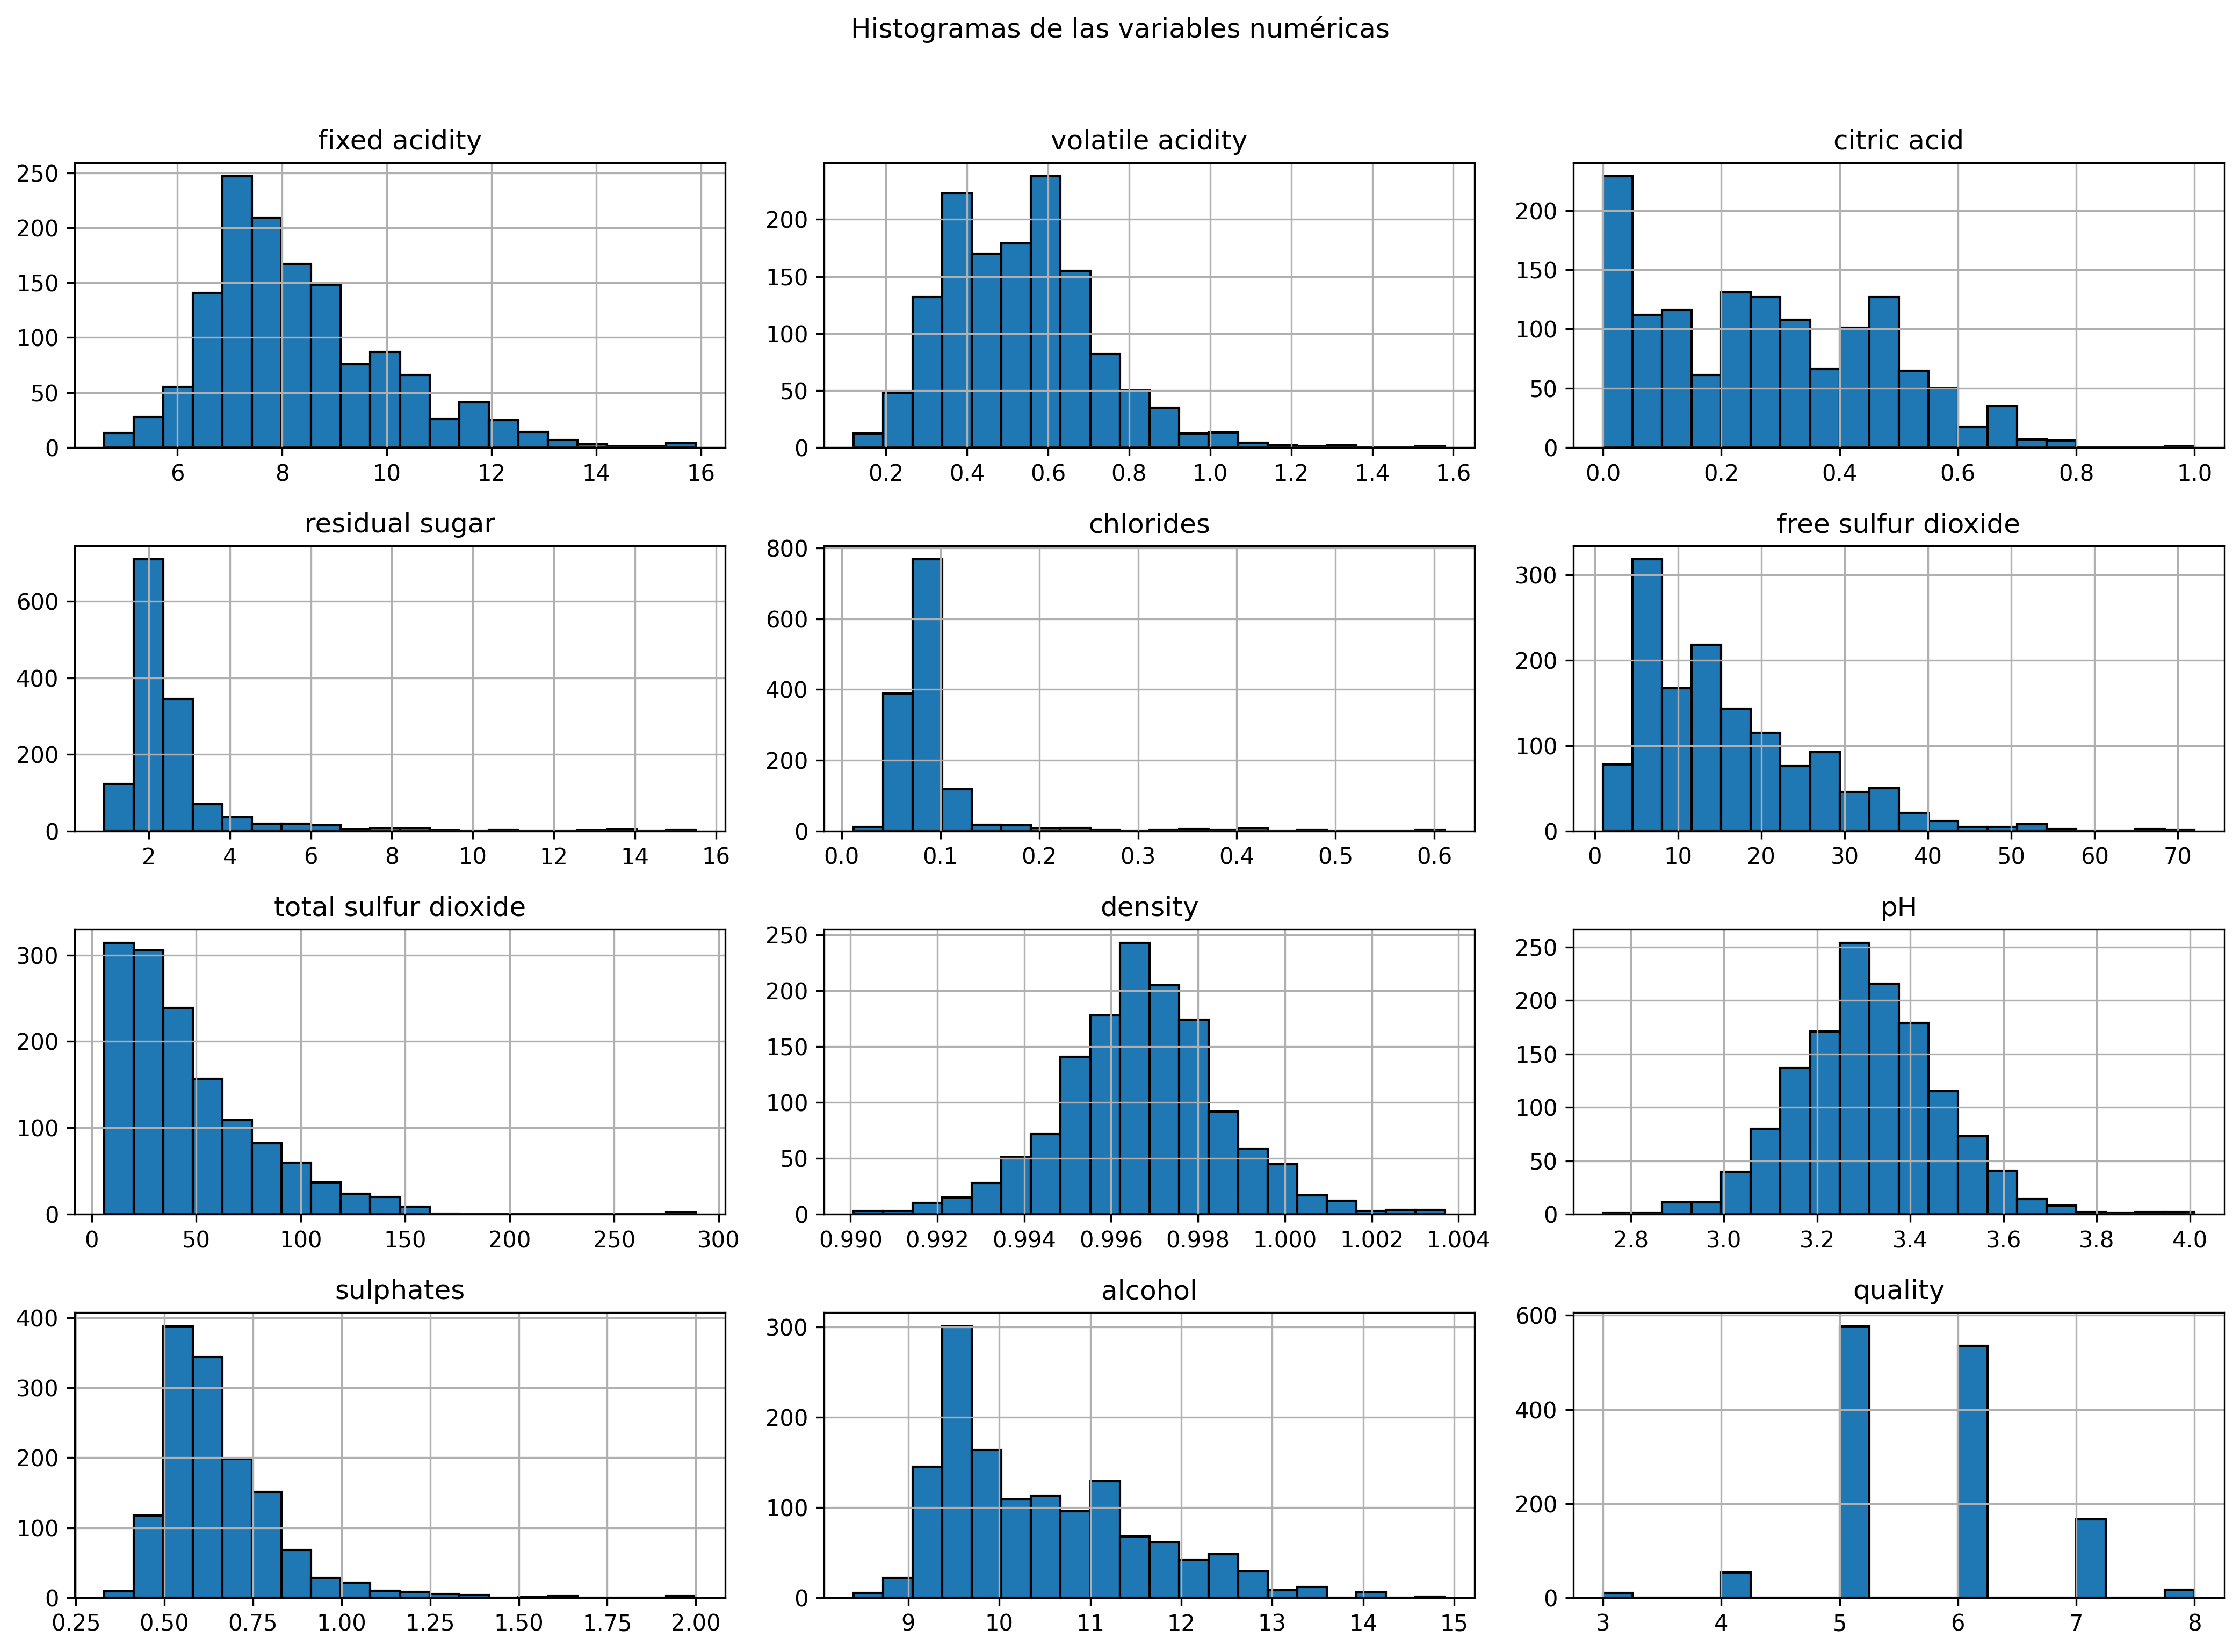
\includegraphics[width=\linewidth]{notebook_md_37_0.png}
    \caption{Histogramas de las variables numéricas del dataset.}
    \label{fig:hist}
\end{figure}

A partir de los histogramas se observó que las variables \textit{density} y \textit{pH} presentaban un comportamiento más cercano a una distribución de campana. En cambio, \textit{quality} no mostraba una forma normal, lo cual es lógico porque se trata de una variable discreta. Varias de las demás variables presentaron sesgo hacia la derecha, especialmente aquellas donde luego también se identificaron outliers en los boxplots.

\subsection{Diagramas de caja}

Los diagramas de caja fueron utilizados para identificar dispersión y valores atípicos en cada una de las variables.

\begin{lstlisting}[caption={Generación de boxplots}, label={lst:boxplots}]
import matplotlib.pyplot as plt
import seaborn as sns

columnas = df.drop(columns=["quality_binary"]).columns

fig, axes = plt.subplots(nrows=4, ncols=3, figsize=(16, 14))
axes = axes.flatten()

for i, col in enumerate(columnas):
    sns.boxplot(x=df[col], ax=axes[i])
    axes[i].set_title(f"{col}")
    axes[i].set_xlabel("")

for j in range(i + 1, len(axes)):
    fig.delaxes(axes[j])

plt.suptitle("Boxplots de las variables numéricas", fontsize=16)
plt.tight_layout()
plt.show()
\end{lstlisting}

\begin{figure}[H]
    \centering
    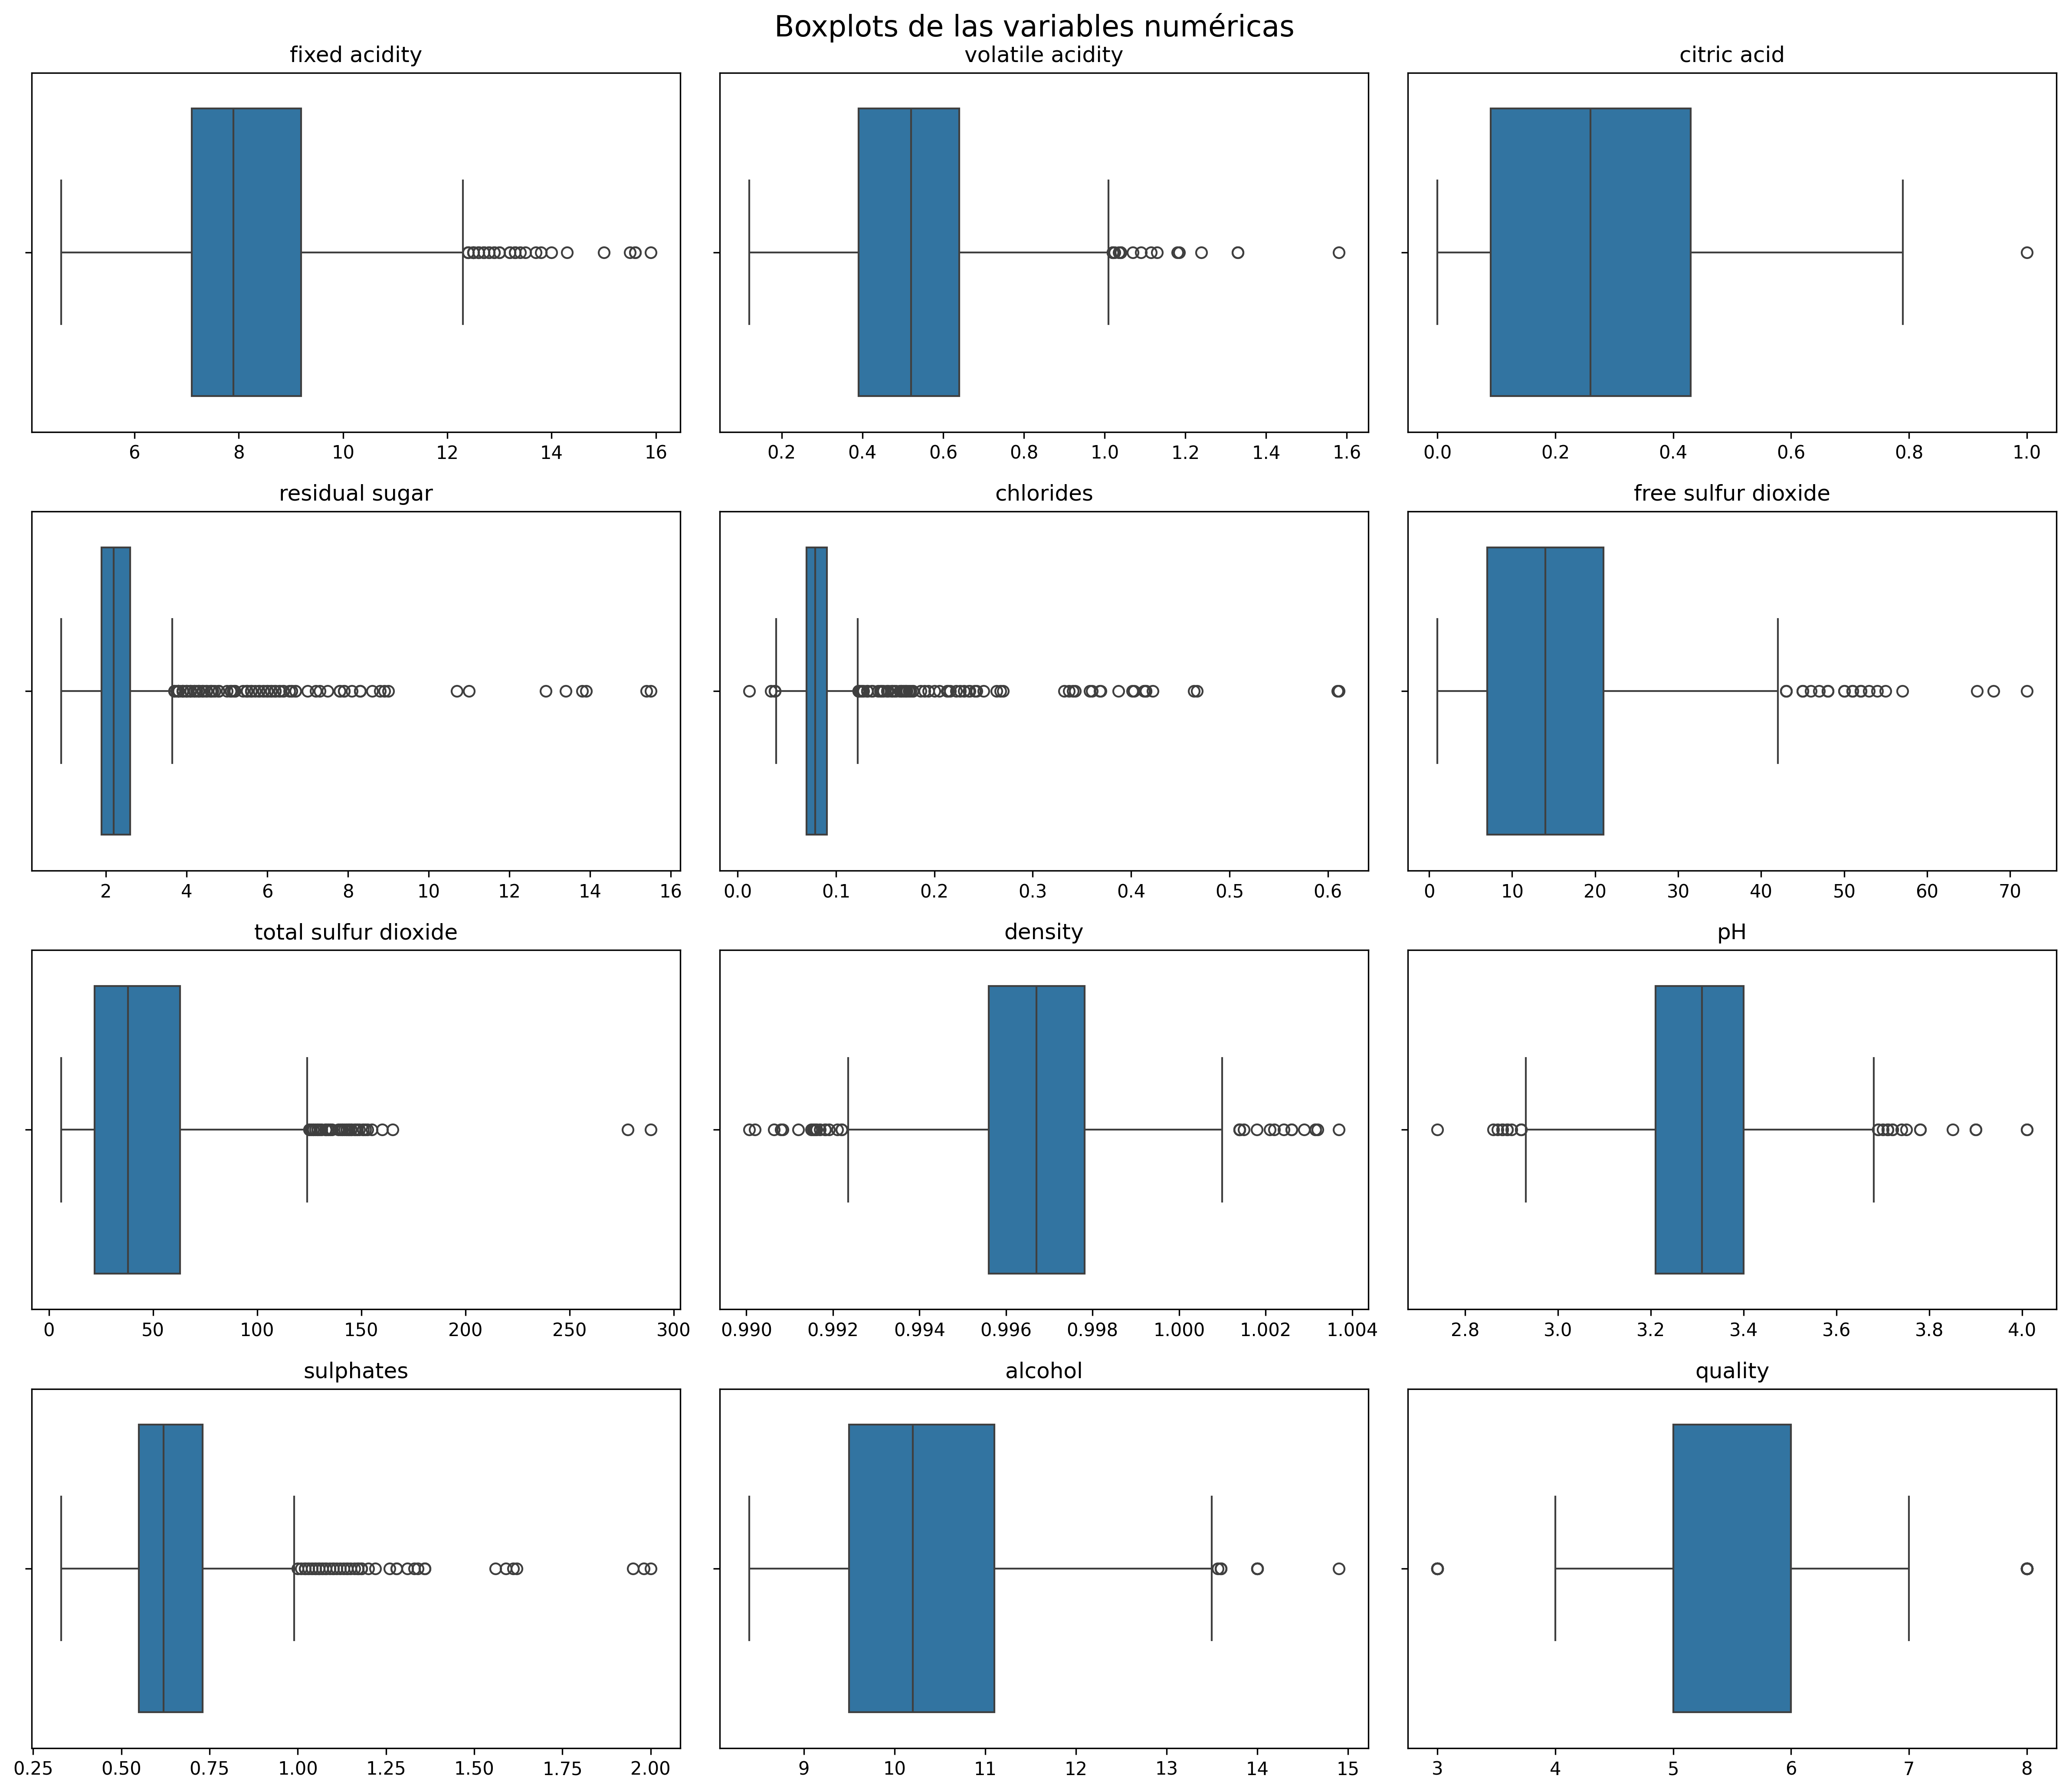
\includegraphics[width=\linewidth]{notebook_md_45_0.png}
    \caption{Boxplots de las variables numéricas del dataset.}
    \label{fig:boxplots}
\end{figure}

En los boxplots se encontró que variables como \textit{residual sugar}, \textit{chlorides}, \textit{free sulfur dioxide}, \textit{total sulfur dioxide} y \textit{sulphates} presentaban una cantidad importante de valores atípicos hacia valores altos. Por otro lado, \textit{density} y \textit{pH} mostraron distribuciones más compactas, aunque no completamente libres de extremos.

\subsection{Diagramas de dispersión respecto a la variable objetivo}

Después se construyeron diagramas de dispersión para visualizar cómo se relacionaba cada característica con la variable objetivo binaria.

\begin{lstlisting}[caption={Diagramas de dispersión respecto al target}, label={lst:scatter}]
import matplotlib.pyplot as plt
import seaborn as sns
import math

target = "quality_binary"
features = [col for col in df.columns if col != target]

n = len(features)
cols = 3
rows = math.ceil(n / cols)

plt.figure(figsize=(15, 5 * rows))

for i, col in enumerate(features, 1):
    plt.subplot(rows, cols, i)
    sns.scatterplot(data=df, x=col, y=target, hue=target, alpha=0.6)
    plt.title(col)

plt.tight_layout()
plt.show()
\end{lstlisting}

\begin{figure}[H]
    \centering
    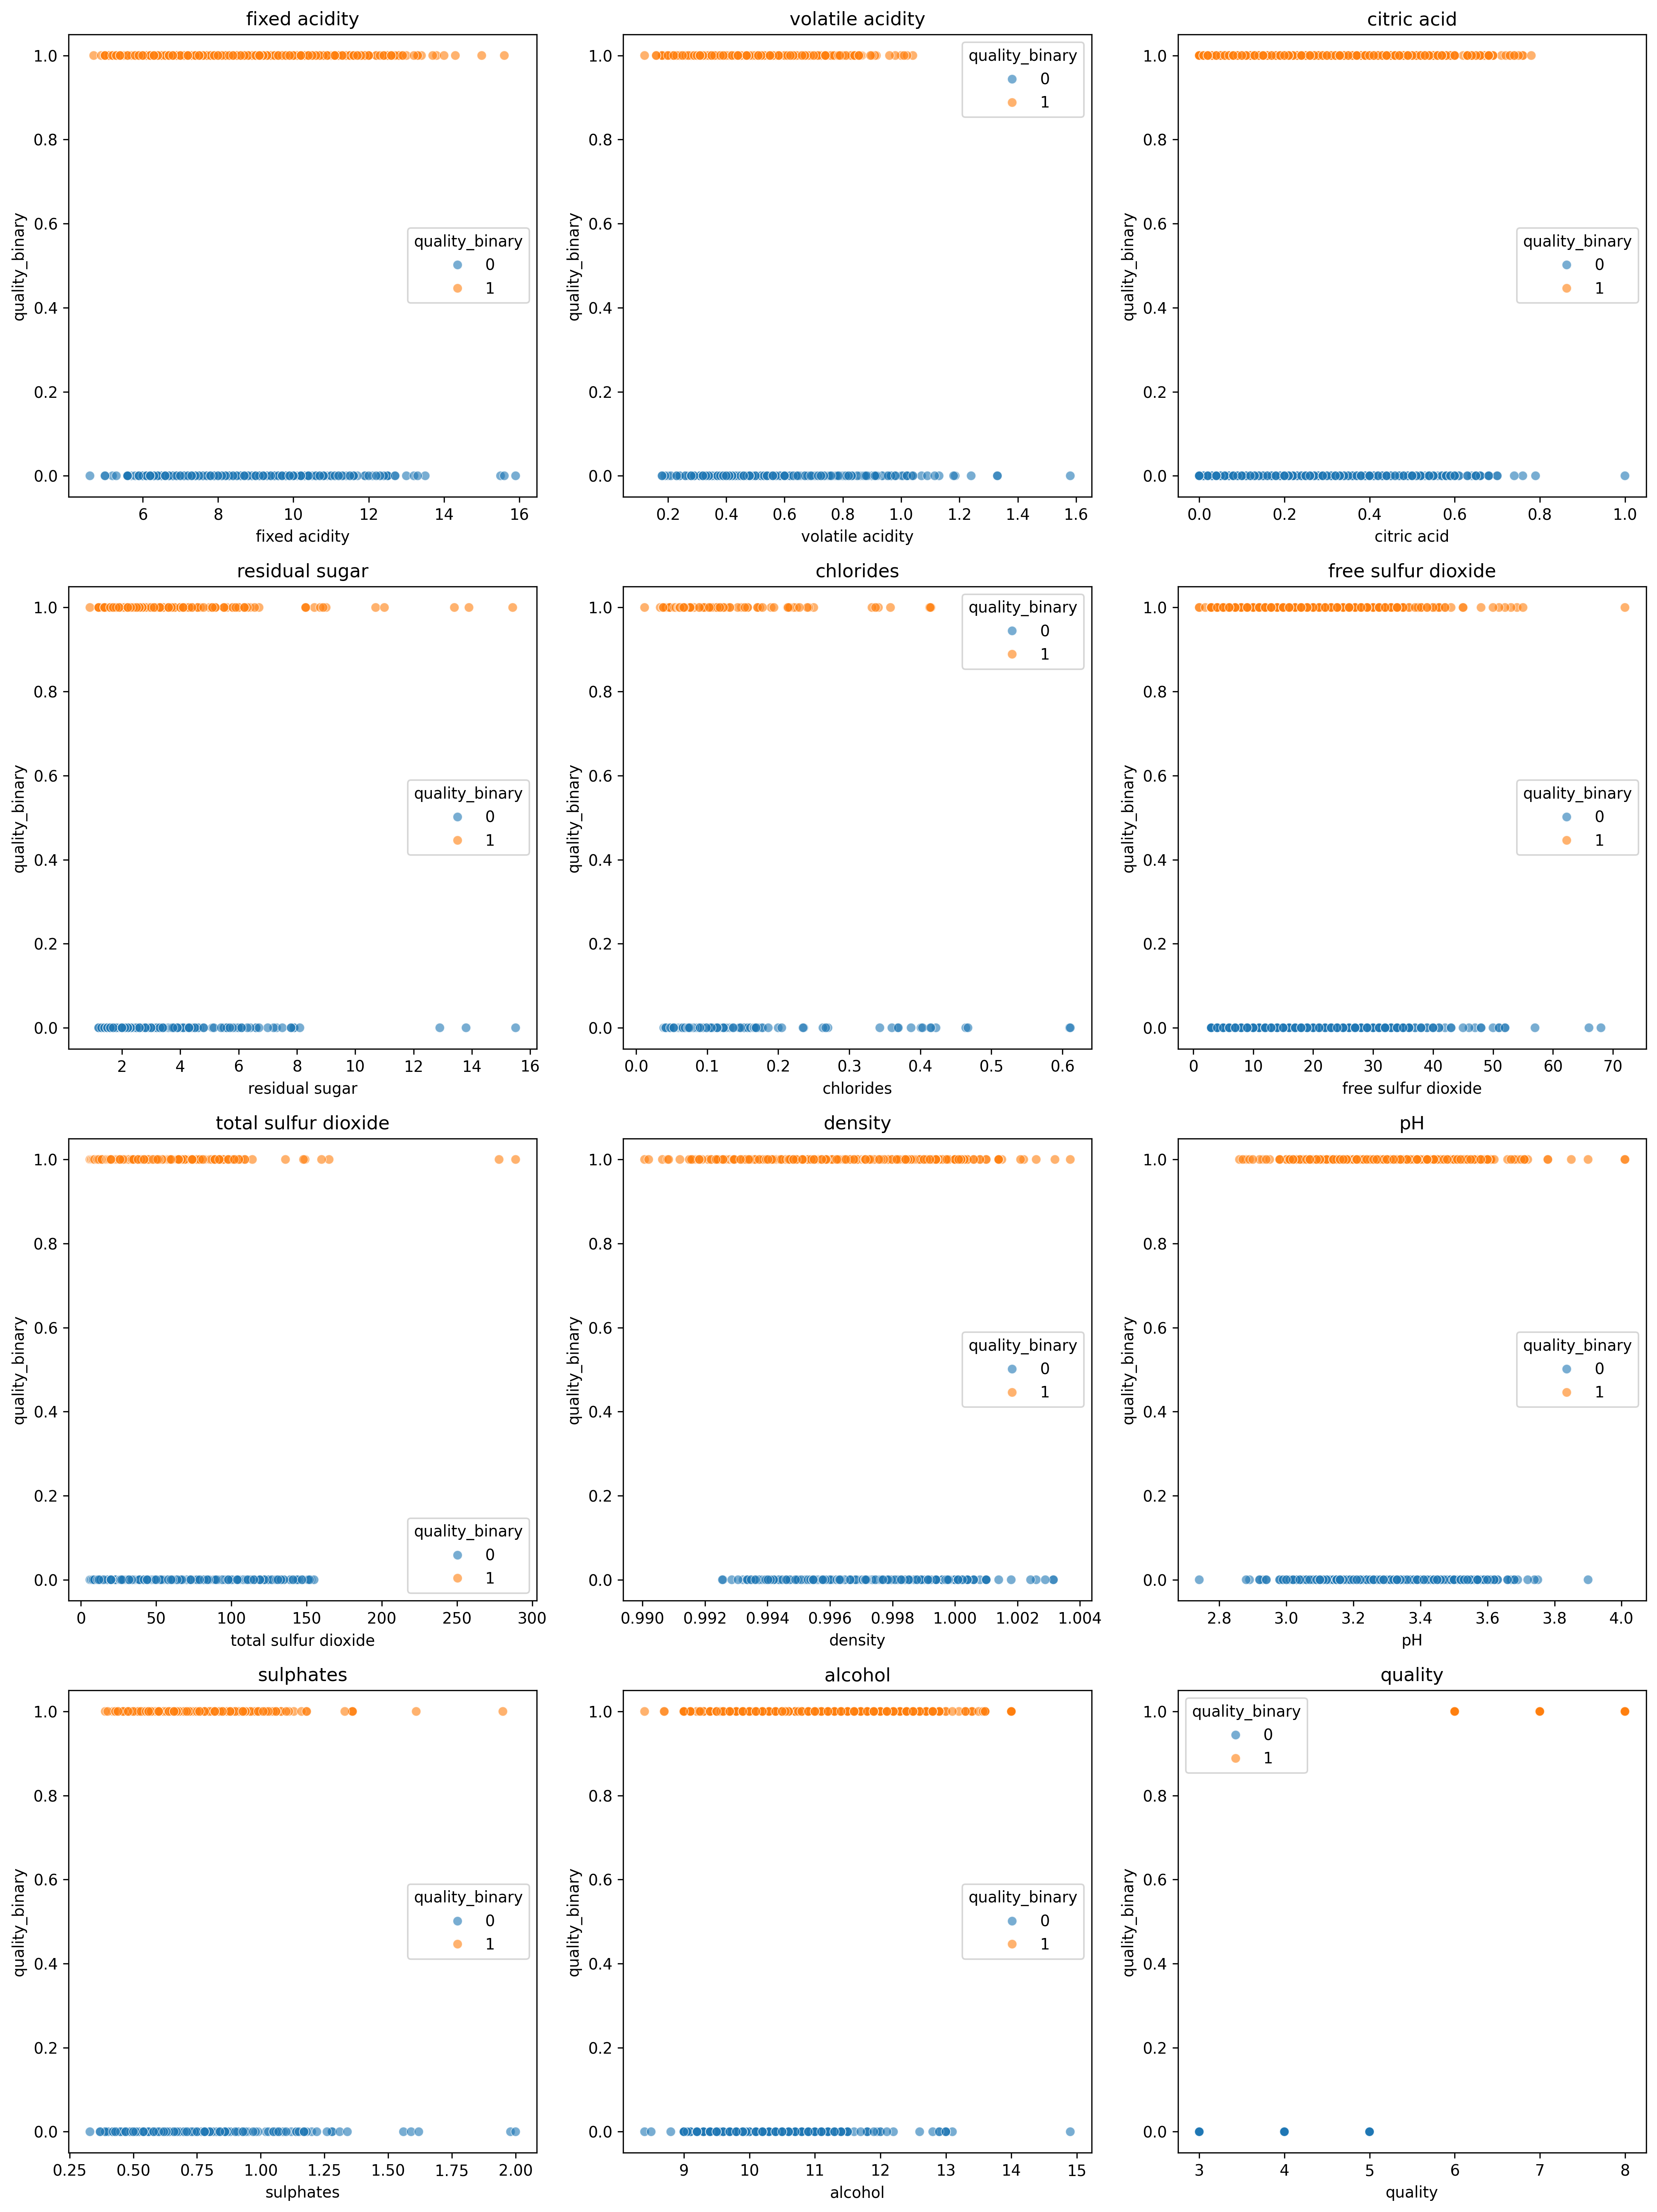
\includegraphics[width=\linewidth]{notebook_md_49_0.png}
    \caption{Diagramas de dispersión de las variables respecto a \texttt{quality\_binary}.}
    \label{fig:scatter}
\end{figure}

En esta visualización se apreció que variables como \textit{alcohol} y \textit{volatile acidity} mostraban una separación más visible entre las clases. Eso sugirió que podían ser especialmente útiles para la predicción. Además, se confirmó nuevamente la presencia de valores extremos en variables como \textit{residual sugar} y \textit{chlorides}. Debido a ello se decidió aplicar posteriormente un tratamiento de outliers mediante IQR.

\subsection{Matriz de correlación}

Para complementar el análisis, se calculó una matriz de correlación y se representó mediante un mapa de calor.

\begin{lstlisting}[caption={Matriz de correlación con mapa de calor}, label={lst:heatmap}]
import matplotlib.pyplot as plt
import seaborn as sns

plt.figure(figsize=(12, 8))
corr = df.corr(numeric_only=True)

sns.heatmap(corr, annot=True, cmap="coolwarm",
            fmt=".2f", linewidths=0.5)
plt.title("Matriz de correlación")
plt.tight_layout()
plt.show()
\end{lstlisting}

\begin{figure}[H]
    \centering
    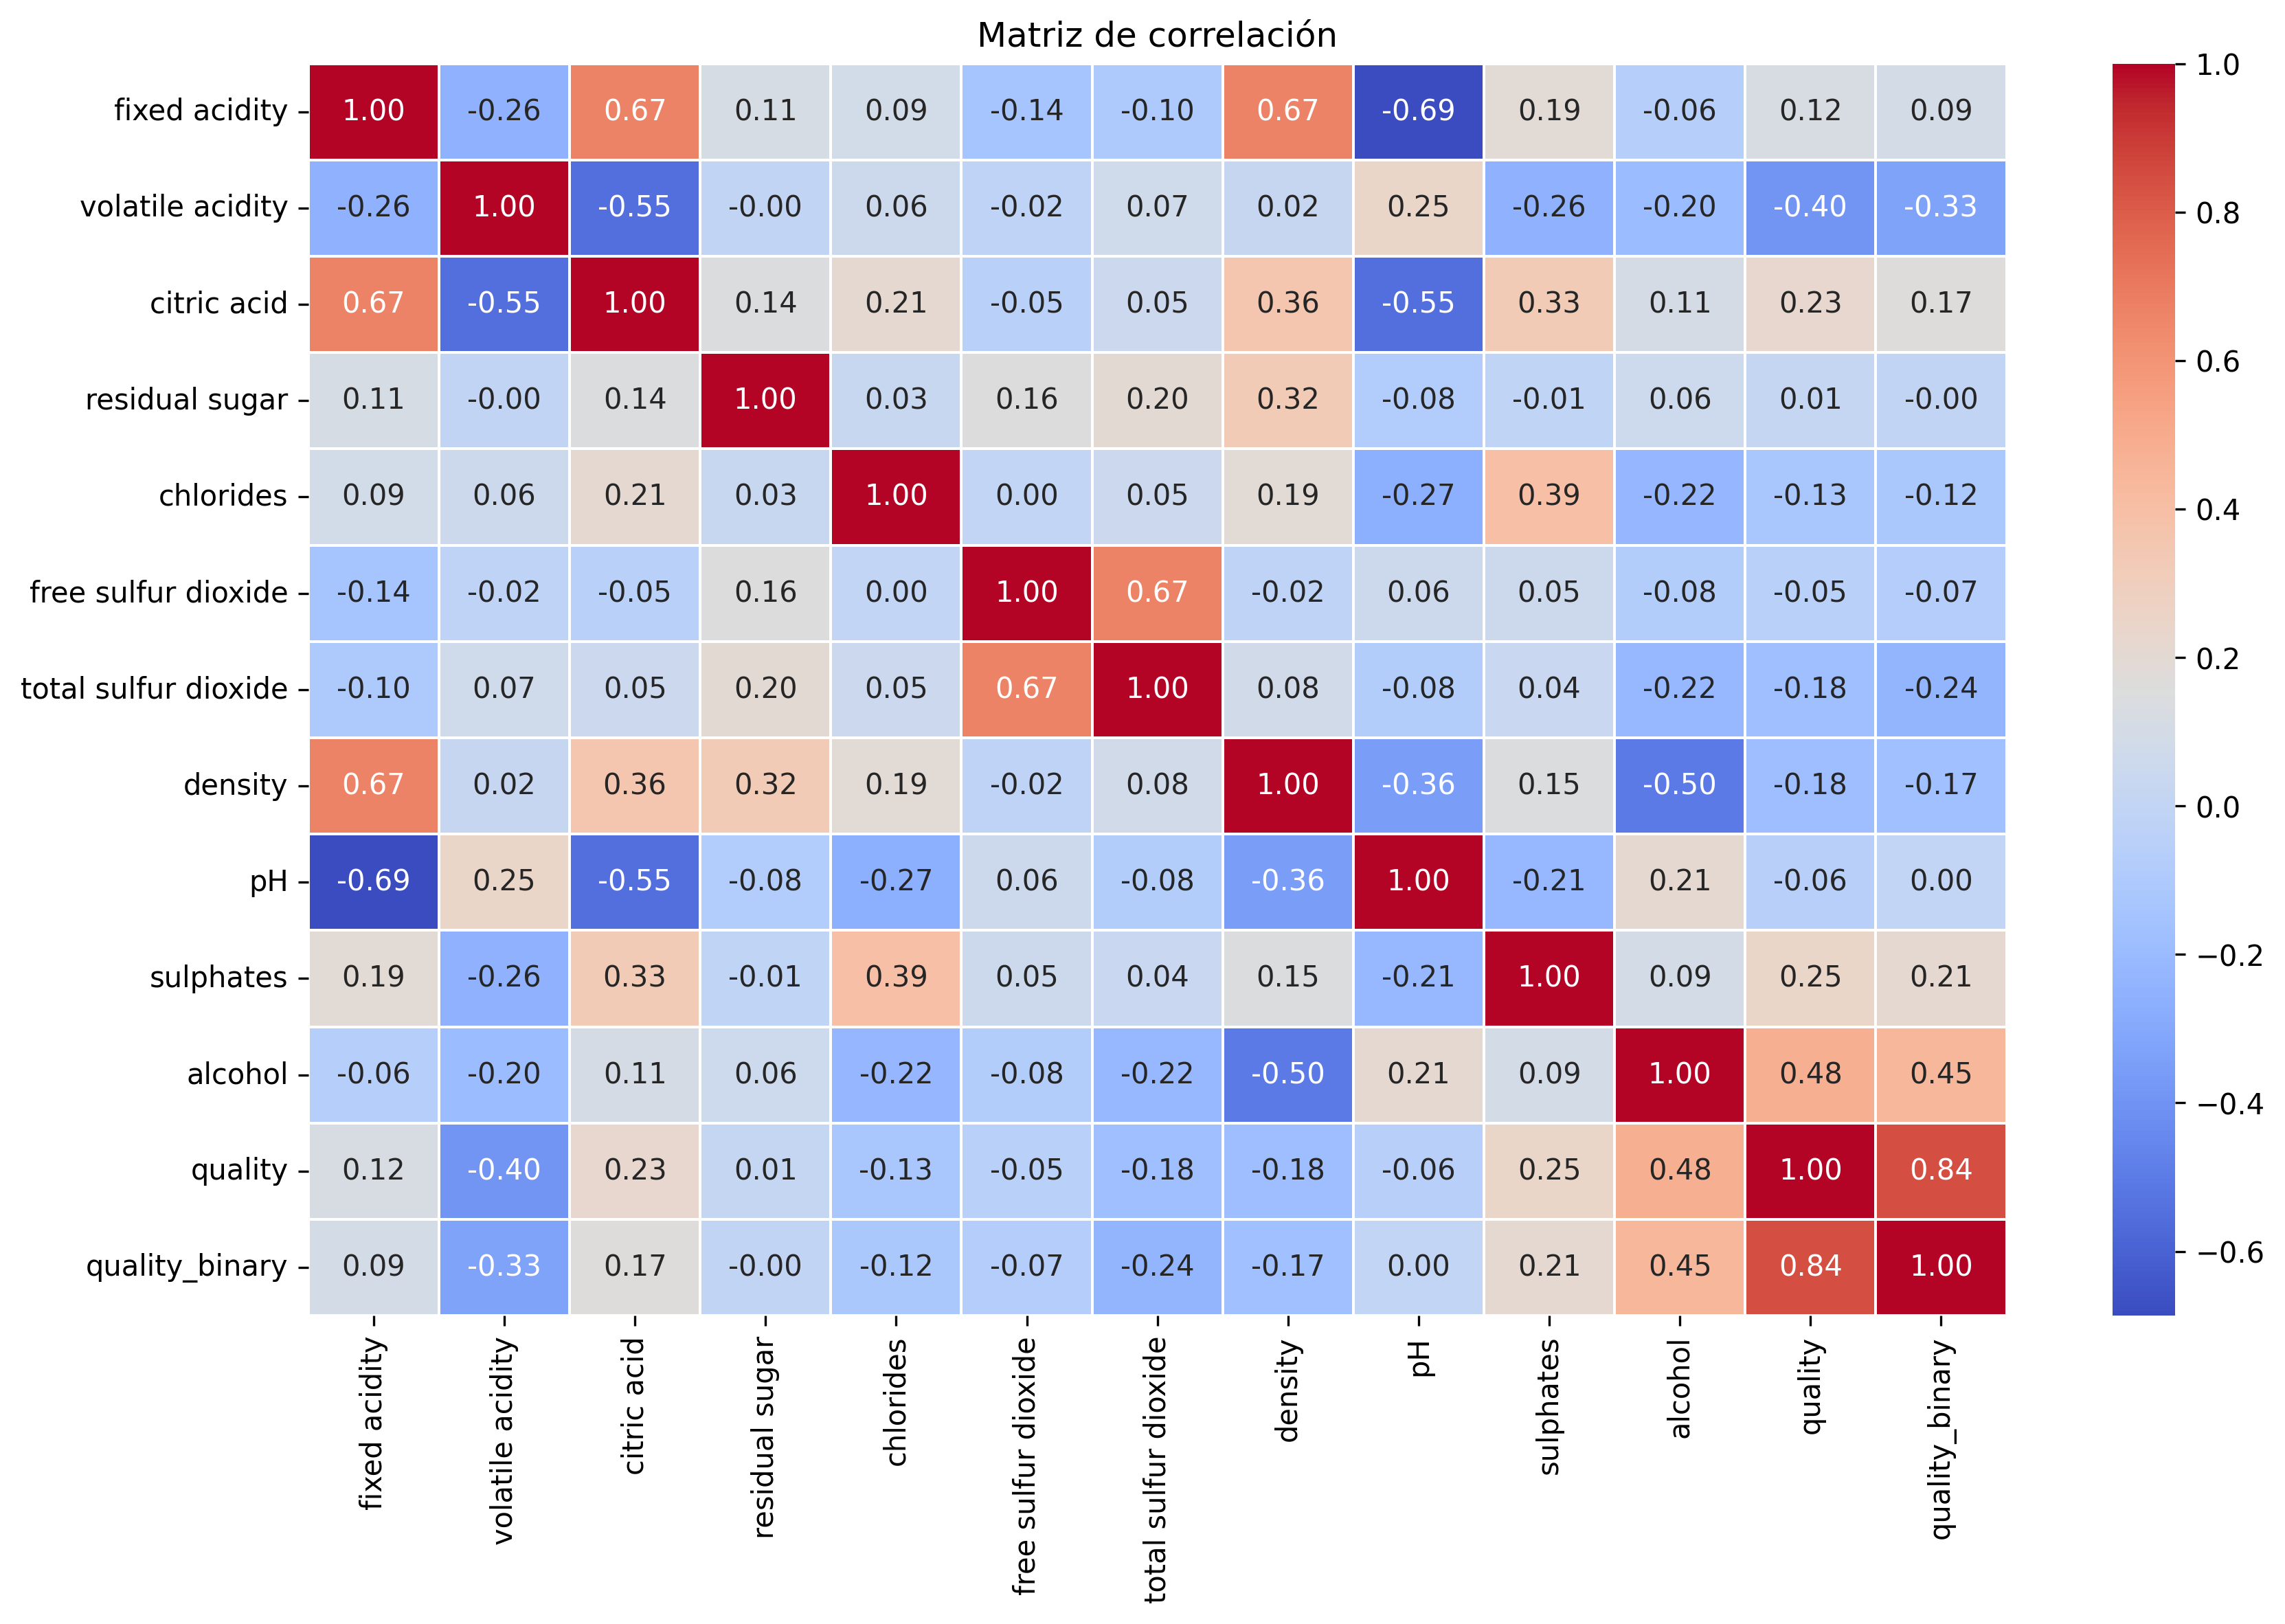
\includegraphics[width=\linewidth]{notebook_md_54_0.png}
    \caption{Mapa de calor de la matriz de correlación.}
    \label{fig:heatmap}
\end{figure}

La matriz mostró que \textit{alcohol} era la variable con mayor correlación positiva respecto a \texttt{quality\_binary}, con un valor de 0.45. En cambio, \textit{volatile acidity} presentó una correlación negativa moderada de aproximadamente -0.33. También destacaron \textit{total sulfur dioxide} con -0.24 y \textit{sulphates} con 0.21.

Además, se observaron correlaciones importantes entre variables predictoras, por ejemplo entre \textit{fixed acidity} y \textit{citric acid} (0.67), \textit{fixed acidity} y \textit{density} (0.67), \textit{free sulfur dioxide} y \textit{total sulfur dioxide} (0.67), y una correlación negativa fuerte entre \textit{fixed acidity} y \textit{pH} (-0.69). Esto sugirió que algunas variables podían aportar información redundante.

\subsection{Selección de las seis variables principales}

Para la selección de características se utilizó como criterio principal el coeficiente de correlación de Pearson entre cada variable numérica y la variable objetivo que se eligió anteriormente. 

\begin{lstlisting}[caption={Búsqueda de variables con mayor correlación}, label={lst:corrtarget}]
corr_target = df.drop(columns=["quality"]).corr(numeric_only=True)["quality_binary"] \
    .drop("quality_binary") \
    .sort_values(key=lambda s: s.abs(), ascending=False)

print(corr_target)
\end{lstlisting}

Se seleccionaron las seis variables con mayor valor absoluto de correlación: \textit{alcohol} (0.435), \textit{volatile acidity} (-0.321), \textit{total sulfur dioxide} (-0.232), \textit{sulphates} (0.218), \textit{citric acid} (0.159) y \textit{density} (-0.159). Las demás variables fueron descartadas por presentar una relación más débil con la variable a predecir. Curiosamente esto concuerda con lo que se vio en la matriz de correlación y los distintos diagramas.

\begin{lstlisting}[caption={Selección final de las seis características}, label={lst:features}]
selected_features = [
    "alcohol",
    "volatile acidity",
    "total sulfur dioxide",
    "sulphates",
    "density",
    "citric acid"
]
\end{lstlisting}

\begin{table}[H]
\centering
\caption{Seis variables seleccionadas según correlación absoluta con \texttt{quality\_binary}}
\label{tab:features}
\begin{tabular}{lc}
\toprule
Variable & Correlación \\
\midrule
alcohol & 0.434751 \\
volatile acidity & -0.321441 \\
total sulfur dioxide & -0.231963 \\
sulphates & 0.218072 \\
citric acid & 0.159129 \\
density & -0.159110 \\
\bottomrule
\end{tabular}
\end{table}

\section{División y preparación de los datos}

\subsection{División estratificada del dataset}

Una vez definidas las seis características principales, el conjunto fue separado en entrenamiento, validación y prueba utilizando muestreo estratificado. Primero se apartó un 70 \% para entrenamiento y un 30 \% temporal, el cual luego fue dividido por igual para validación y prueba.

\begin{lstlisting}[caption={División del dataset en entrenamiento, validación y prueba}, label={lst:split}]
from sklearn.model_selection import train_test_split

selected_features = [
    "alcohol",
    "volatile acidity",
    "total sulfur dioxide",
    "sulphates",
    "density",
    "citric acid"
]

X = df[selected_features]
y = df["quality_binary"]

# 70% entrenamiento, 30% temporal
X_train, X_temp, y_train, y_temp = train_test_split(
    X, y,
    test_size=0.30,
    stratify=y,
    random_state=42
)

# 15% validación, 15% prueba
X_val, X_test, y_val, y_test = train_test_split(
    X_temp, y_temp,
    test_size=0.50,
    stratify=y_temp,
    random_state=42
)
\end{lstlisting}

Las proporciones de clase se mantuvieron prácticamente iguales en los tres subconjuntos, lo que indicó que el proceso de estratificación fue correcto y ayudó a evitar sesgos en la evaluación.

\subsection{Aplicación del método IQR}

Como el análisis exploratorio mostró presencia de outliers, se decidió aplicar una estrategia de capado usando el rango intercuartílico (IQR). Este procedimiento se calculó únicamente con el conjunto de entrenamiento para evitar fuga de información.

\begin{lstlisting}[caption={Tratamiento de outliers con IQR}, label={lst:iqr}]
X_train_iqr = X_train.copy()
X_val_iqr = X_val.copy()
X_test_iqr = X_test.copy()

for col in selected_features:
    Q1 = X_train[col].quantile(0.25)
    Q3 = X_train[col].quantile(0.75)
    IQR = Q3 - Q1

    lower = Q1 - 1.5 * IQR
    upper = Q3 + 1.5 * IQR

    X_train_iqr[col] = X_train_iqr[col].clip(lower, upper)
    X_val_iqr[col] = X_val_iqr[col].clip(lower, upper)
    X_test_iqr[col] = X_test_iqr[col].clip(lower, upper)
\end{lstlisting}

Este enfoque permitió limitar los valores extremos sin necesidad de eliminar filas completas.

\subsection{Escalado de los datos}

Posteriormente, las variables fueron estandarizadas usando \texttt{StandardScaler}. Esta etapa fue importante porque las características tenían rangos distintos, y la regresión logística puede verse afectada si unas variables dominan a otras por escala.

\begin{lstlisting}[caption={Escalado de las variables con StandardScaler}, label={lst:scaler}]
from sklearn.preprocessing import StandardScaler

scaler = StandardScaler()

X_train_scaled = scaler.fit_transform(X_train_iqr)
X_val_scaled = scaler.transform(X_val_iqr)
X_test_scaled = scaler.transform(X_test_iqr)
\end{lstlisting}

\section{Implementación con PyTorch}

\subsection{Conversión de datos a tensores}

Una vez escaladas las entradas, los subconjuntos se transformaron a tensores de PyTorch para poder utilizarlos dentro del modelo.

\begin{lstlisting}[caption={Conversión de datos a tensores}, label={lst:tensors}]
import torch

X_train_tensor = torch.tensor(X_train_scaled, dtype=torch.float32)
X_val_tensor = torch.tensor(X_val_scaled, dtype=torch.float32)
X_test_tensor = torch.tensor(X_test_scaled, dtype=torch.float32)

y_train_tensor = torch.tensor(y_train.values,
                              dtype=torch.float32).view(-1, 1)
y_val_tensor = torch.tensor(y_val.values,
                            dtype=torch.float32).view(-1, 1)
y_test_tensor = torch.tensor(y_test.values,
                             dtype=torch.float32).view(-1, 1)
\end{lstlisting}

\subsection{Creación de los \textit{Dataset} y \textit{DataLoader}}

Con los tensores ya preparados, se construyeron los objetos \texttt{TensorDataset} y \texttt{DataLoader} para organizar el entrenamiento por lotes.

\begin{lstlisting}[caption={Creación de TensorDataset y DataLoader}, label={lst:dataloaders}]
from torch.utils.data import TensorDataset, DataLoader

train_dataset = TensorDataset(X_train_tensor, y_train_tensor)
val_dataset = TensorDataset(X_val_tensor, y_val_tensor)

train_loader = DataLoader(train_dataset, batch_size=32, shuffle=True)
val_loader = DataLoader(val_dataset, batch_size=32, shuffle=False)
\end{lstlisting}

\subsection{Definición del modelo de regresión logística}

El modelo se implementó como una sola capa lineal, adecuada para clasificación binaria.

\begin{lstlisting}[caption={Definición del modelo de regresión logística en PyTorch}, label={lst:modelo}]
import torch.nn as nn

class LogisticRegressionModel(nn.Module):
    def __init__(self, input_dim):
        super().__init__()
        self.linear = nn.Linear(input_dim, 1)

    def forward(self, x):
        return self.linear(x)
\end{lstlisting}

\section{Ejecución de los diez experimentos}

\subsection{Configuración de experimentos}

Para comparar distintas configuraciones, se definieron diez experimentos variando tasa de aprendizaje, tamaño de batch y número de épocas.

\begin{lstlisting}[caption={Definición de los diez experimentos}, label={lst:experiments}]
experiments = [
    {"lr": 0.001, "batch": 16, "epochs": 20},
    {"lr": 0.001, "batch": 32, "epochs": 20},
    {"lr": 0.001, "batch": 64, "epochs": 20},
    {"lr": 0.005, "batch": 16, "epochs": 20},
    {"lr": 0.005, "batch": 32, "epochs": 20},
    {"lr": 0.005, "batch": 64, "epochs": 20},
    {"lr": 0.01,  "batch": 16, "epochs": 20},
    {"lr": 0.01,  "batch": 32, "epochs": 20},
    {"lr": 0.01,  "batch": 64, "epochs": 20},
    {"lr": 0.01,  "batch": 32, "epochs": 50},
]
\end{lstlisting}

\subsection{Loop de entrenamiento y captura de métricas}

En esta sección se procedió con la ejecución de los experimentos. Se integró un diccionario para capturar el historial de la función de pérdida (\textit{Loss}) en cada época, con el fin de graficar posteriormente las curvas de aprendizaje.

\begin{lstlisting}[caption={Ejecución de los diez entrenamientos y almacenamiento de Loss}, label={lst:10runs}]
import torch.optim as optim
from sklearn.metrics import accuracy_score, precision_score, recall_score, f1_score, roc_auc_score

results = []
loss_history = {} 

criterion = nn.BCEWithLogitsLoss()

for i, exp in enumerate(experiments): 
    # instanciar el modelo y el optimizador
    model = LogisticRegressionModel(input_dim=X_train_tensor.shape[1])
    optimizer = optim.Adam(model.parameters(), lr=exp["lr"])
    
    # configurar el dataloader
    train_loader = DataLoader(train_dataset, batch_size=exp["batch"], shuffle=True)
    
    train_losses = []
    val_losses = []
    
    # ciclo de entrenamiento (epochs)
    for epoch in range(exp["epochs"]):
        model.train()
        epoch_train_loss = 0
        
        for batch_X, batch_y in train_loader:
            optimizer.zero_grad()
            outputs = model(batch_X)
            
            # forzamos que el target sea [Batch, 1]
            batch_y_correct = batch_y.view(-1, 1).float()
            loss = criterion(outputs, batch_y_correct)
            
            loss.backward()
            optimizer.step()
            epoch_train_loss += loss.item()
            
        train_losses.append(epoch_train_loss / len(train_loader))
        
        # evaluacion en validacion para la curva
        model.eval()
        with torch.no_grad():
            val_outputs = model(X_val_tensor)
            y_val_correct = y_val_tensor.view(-1, 1).float()
            val_loss = criterion(val_outputs, y_val_correct)
            val_losses.append(val_loss.item())
            
    # guardar el historial para graficas
    loss_history[f"Exp_{i+1}"] = {"train": train_losses, "val": val_losses}
    
    # evaluacion final para metricas comparativas
    model.eval()
    with torch.no_grad():
        logits = model(X_val_tensor)
        probs = torch.sigmoid(logits).numpy().flatten()
        preds = (probs >= 0.5).astype(int)
        
    y_true = y_val_tensor.numpy()
    
    results.append({
        "Exp": i+1,
        "LR": exp["lr"],
        "Batch": exp["batch"],
        "Epochs": exp["epochs"],
        "Accuracy": accuracy_score(y_true, preds),
        "Precision": precision_score(y_true, preds, zero_division=0),
        "Recall": recall_score(y_true, preds, zero_division=0),
        "F1": f1_score(y_true, preds, zero_division=0),
        "AUC": roc_auc_score(y_true, probs)
    })

results_df = pd.DataFrame(results)
\end{lstlisting}

\vspace{-10mm}
\begin{table}[H]
\centering
\caption{Resultados de los 10 experimentos ordenados por F1 sobre validación}
\label{tab:experimentos}
\scriptsize
\resizebox{\linewidth}{!}{
\begin{tabular}{ccccccccc}
\toprule
Exp & LR & Batch & Epochs & Accuracy & Precision & Recall & F1 & AUC \\
\midrule
2 & 0.001 & 32 & 20 & 0.7402 & 0.7778 & 0.7130 & 0.7440 & 0.8234 \\
10 & 0.010 & 32 & 50 & 0.7206 & 0.7629 & 0.6852 & 0.7220 & 0.8286 \\
6 & 0.005 & 64 & 20 & 0.7157 & 0.7500 & 0.6944 & 0.7212 & 0.8202 \\
7 & 0.010 & 16 & 20 & 0.7157 & 0.7551 & 0.6852 & 0.7184 & 0.8277 \\
9 & 0.010 & 64 & 20 & 0.7108 & 0.7475 & 0.6852 & 0.7150 & 0.8264 \\
8 & 0.010 & 32 & 20 & 0.7108 & 0.7475 & 0.6852 & 0.7150 & 0.8294 \\
5 & 0.005 & 32 & 20 & 0.7059 & 0.7400 & 0.6852 & 0.7115 & 0.8273 \\
4 & 0.005 & 16 & 20 & 0.7059 & 0.7400 & 0.6852 & 0.7115 & 0.8269 \\
1 & 0.001 & 16 & 20 & 0.6961 & 0.7300 & 0.6759 & 0.7019 & 0.8252 \\
3 & 0.001 & 64 & 20 & 0.6618 & 0.7191 & 0.5926 & 0.6497 & 0.7052 \\
\bottomrule
\end{tabular}
}
\end{table}
\vspace{-4mm}

\subsection{Curvas de Aprendizaje}

Al graficar el historial guardado en el paso anterior, se contrastó el error de entrenamiento frente al error de validación para detectar problemas de generalización.

\begin{figure}[H]
    \centering
    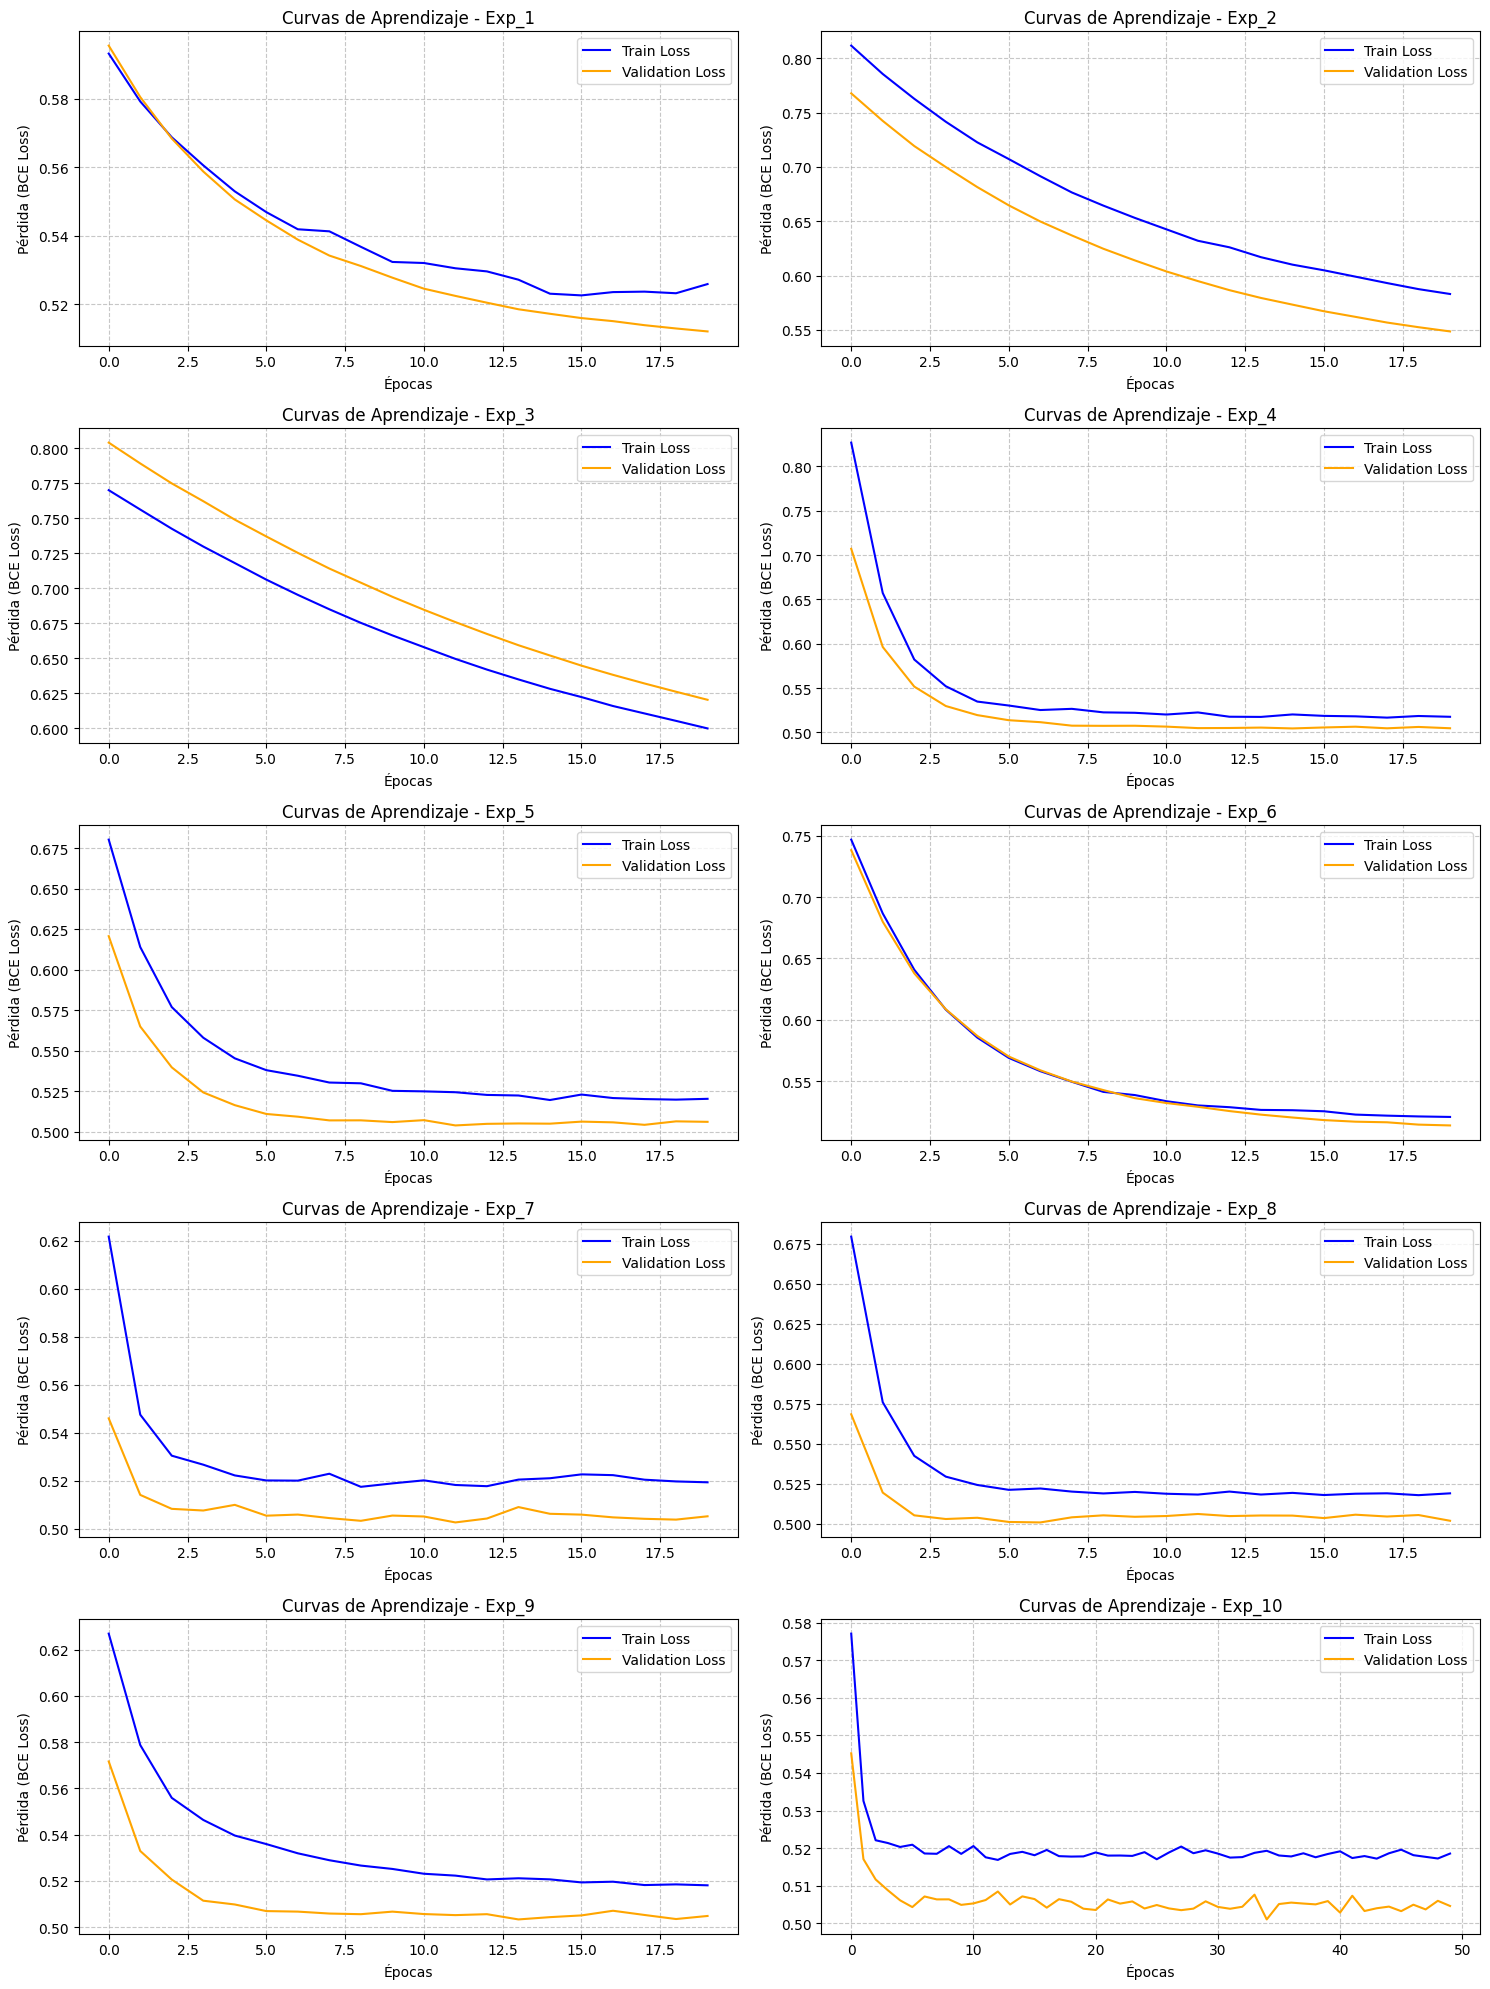
\includegraphics[width=\linewidth]{curvas_aprendizaje.png}
    \caption{Gráficas de curvas de aprendizaje (Loss) para cada experimento.}
    \label{fig:curvas}
\end{figure}

El aspecto más destacable es el comportamiento de la curva de validación, la cual acompañó estrechamente el descenso de la curva de entrenamiento. El hecho de que el \textit{Validation Loss} disminuyera y se estabilizara a la par del \textit{Train Loss}, sin presentar repuntes abruptos o divergencias hacia el final de las épocas, es un indicador empírico sólido de que los modelos no sufrieron de sobreajuste (\textit{overfitting}).

\section{Análisis de resultados y Selección del modelo}

A partir del cuadro comparativo (Tabla \ref{tab:experimentos}), se observó una varianza significativa en el rendimiento de los modelos. El \textbf{Experimento 2} destacó de manera contundente como el mejor modelo general. No solo obtuvo el máximo F1-Score (0.7440), sino que lideró casi todas las métricas de clasificación directa: Exactitud (0.7402), Precisión (0.7778) y Recall (0.7130). Su configuración ($LR = 0.001$, $Batch = 32$, $Epochs = 20$) logró el mejor punto de convergencia.

Se evidencia que un tamaño de lote de 32 fue el punto óptimo para este conjunto de datos, ya que los experimentos que lo utilizaron dominan la parte superior de la tabla. Por el contrario, tamaños de lote más grandes generaron actualizaciones de gradiente menos precisas, desplomando las métricas. Basado en esta evidencia cuantitativa, se seleccionó oficialmente el \textbf{Experimento 2} como el modelo definitivo.

\subsection{Evaluación Final con Conjunto de Prueba (Testing Set)}

Para comprobar la capacidad real de generalización, se procedió a re-entrenar el modelo con la configuración ganadora y a evaluarlo utilizando el conjunto de prueba (Test Set).

\begin{lstlisting}[caption={Re-entrenamiento y evaluación con el conjunto de pruebas}, label={lst:testing}]
# configuracion del modelo ganador
mejor_lr = 0.001
mejor_batch = 32
mejores_epochs = 20

modelo_final = LogisticRegressionModel(input_dim=X_train_tensor.shape[1])
optimizador_final = optim.Adam(modelo_final.parameters(), lr=mejor_lr)
criterio_final = nn.BCEWithLogitsLoss()

train_loader_final = DataLoader(train_dataset, batch_size=mejor_batch, shuffle=True)

# entrenamiento final
modelo_final.train()
for epoch in range(mejores_epochs):
    for batch_X, batch_y in train_loader_final:
        optimizador_final.zero_grad()
        outputs = modelo_final(batch_X)
        loss = criterio_final(outputs, batch_y.view(-1, 1).float())
        loss.backward()
        optimizador_final.step()

# evaluacion con el conjunto de testing
modelo_final.eval()
with torch.no_grad():
    test_logits = modelo_final(X_test_tensor)
    test_probs = torch.sigmoid(test_logits).numpy().flatten()
    test_preds = (test_probs >= 0.5).astype(int)
\end{lstlisting}

Al someter el modelo óptimo al conjunto de pruebas, se obtuvieron las siguientes métricas de rendimiento final: \textbf{Accuracy de 0.7549}, \textbf{Precision de 0.7900}, \textbf{Recall de 0.7315}, \textbf{F1-Score de 0.7596} y un \textbf{AUC de 0.8273}. 

Al comparar estos resultados finales con los obtenidos durante la fase de validación (donde el F1-Score fue de 0.7440), se observó que no solo no hubo degradación del rendimiento, sino que el modelo logró una leve mejora en su capacidad de generalización. 

\begin{figure}[H]
    \centering
    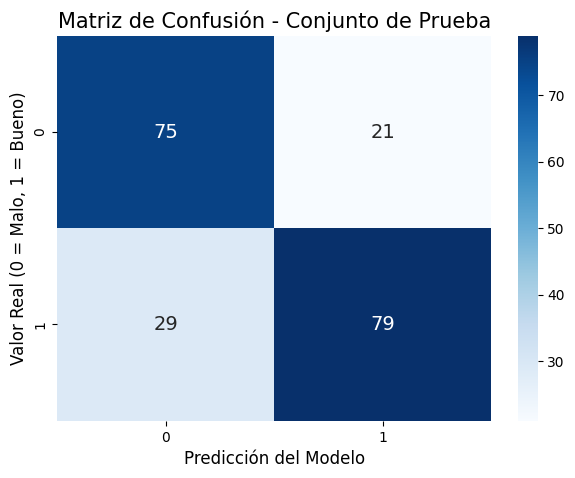
\includegraphics[width=0.8\linewidth]{matriz_confusion.png}
    \caption{Matriz de confusión obtenida al evaluar el conjunto de pruebas.}
    \label{fig:confusion}
\end{figure}

La matriz de confusión (Figura \ref{fig:confusion}) ofreció una visión detallada de los aciertos y errores sobre un total de 204 muestras en un escenario real. El modelo clasificó de forma correcta 79 vinos de buena calidad (TP) y 75 vinos de baja calidad (TN). Esta alta concentración en la diagonal principal evidenció que las características químicas seleccionadas poseen el peso matemático suficiente para separar ambas clases. La proximidad métrica entre los errores Tipo I (21) y Tipo II (29) demostró un clasificador equilibrado y estable, producto del correcto tratamiento previo y el muestreo estratificado.

\section{Conclusiones}

A partir del análisis exploratorio se determinó que el dataset presentaba una estructura adecuada para trabajar un problema de clasificación binaria, aunque fue necesario eliminar 240 filas duplicadas y tratar valores atípicos mediante el uso del rango intercuartílico (IQR). También se comprobó que no existían valores nulos, lo cual simplificó el preprocesamiento inicial.

La transformación de la variable \texttt{quality} a \texttt{quality\_binary} permitió replantear el problema como una clasificación entre vinos buenos y malos. A partir del estudio de correlación se seleccionaron las seis variables con la relación más fuerte: \textit{alcohol}, \textit{volatile acidity}, \textit{total sulfur dioxide}, \textit{sulphates}, \textit{density} y \textit{citric acid}. 

La implementación con PyTorch permitió construir un modelo de regresión logística y entrenarlo mediante mini-batches, capturando historiales de pérdida que demostraron un descenso saludable sin indicios de sobreajuste.

Finalmente, entre los diez experimentos ejecutados, el modelo definitivo (Experimento 2) no solo se destacó durante la validación, sino que al enfrentarse a datos desconocidos del conjunto de pruebas logró un F1 de 0.7596 y una Exactitud de 0.7549. Esto demuestra que la regresión logística desarrollada en PyTorch cumple satisfactoriamente con el objetivo propuesto de catalogar la calidad del vino basándose de forma exclusiva en su perfil químico.

\section*{Nota importante sobre figuras y cierre del trabajo}

Para compilar correctamente este documento, es necesario que las figuras utilizadas estén en la misma carpeta del archivo \texttt{.tex}. En este caso, los nombres empleados fueron los siguientes:

\begin{verbatim}
notebook_md_37_0.png
notebook_md_45_0.png
notebook_md_49_0.png
notebook_md_54_0.png
curvas_aprendizaje.png
matriz_confusion.png
\end{verbatim}

\end{document}